Nous avons vu que le problème du désassemblage tient dans la difficulté de séparer les parties de codes des parties de données d'un programme binaire.
Dans ce chapitre et dans un premier temps, nous proposons une preuve du caractère indécidable du désassemblage puis expliquerons les différentes techniques de désassemblage. Dans un second temps nous détaillerons notre approche du désassemblage qui permet de traiter le cas des programmes auto-modifiants ainsi que le chevauchement de code.


\paragraph{Difficulté théorique du désassemblage.}
~\\
\idone{Pb de l'arrêt: il existe HALT / pour tout P,I : HALT(P,I) = 1 ssi P(I) termine}
\itodo{Pb du désassemblage : borne min : intersection de CODE(P,I), borne max : union}
\itodo{borne min ~ arrêt ?}
% On a vu que le problème du désassemblage tient dans la difficulté de séparer les parties de code potentiel des parties de données.
Si on cherche à séparer le code des données alors le but du désassemblage d'un programme P est de résoudre le problème suivant. On se limite dans un premier temps à un programme P de taille finie et non auto-modifiant.
\begin{pb}
Soit \adr{a} une adresse, existe-t-il une entrée I de P telle que P(I) atteint \adr{a} ?
\end{pb}


% de déterminer l'ensemble des adresses $a$ du programme pour lesquelles il existe une entrée I telle que l'exécution de P(I) atteint $a$.
Nous citons ici un argument tiré de la thèse de Joan Calvet \cite{Calvet2013} montrant le caractère indécidable de ce problème en réduisant le problème de l'arrêt à celui-ci.

% Supposons que le problème soit décidable et notons $CODE$ le programme tel que, pour tout programme P, $CODE(P)$ est l'ensemble des adresses des instructions de P atteignables lors de l'exécution de P. Pour tout programme P et toute entrée I à P, on peut définir le programme P' suivant qui ne prend pas d'entrée :
Supposons que le problème soit décidable. Notons CODE le programme vérifiant, pour tout programme P et adresse \adr{a}, CODE(P, \adr{a}) = 1 si et seulement si il existe une entrée I de P telle que P(I) atteint \adr{a}. Dans le cas contraire CODE (P, \adr{a}) = 0.
Soit P un programme et I une entrée de P. Prenons P' le programme suivant qui ne prend pas d'entrée : P' = P(I).

% \begin{center}
% \begin{tabular}{|l|l|}
% \hline
% Adresse & Commande \\
% \hline
% 0 & P(I)\\
% % $\alpha$ & halt \\
% \hline
% \end{tabular}
% \end{center}

% On remarque que $CODE(P')$ contient exactement les adresses des instructions de P 
Deux cas sont alors possibles.
\begin{itemize}
 \item Soit il existe une adresse $\alpha$ tel que l'instruction à l'adresse $\alpha$ est l'instruction d'arrêt \texttt{halt} et telle que CODE(P, $\alpha$) = 1 : il existe une entrée I' à P' telle que P'(I') atteint $\alpha$. Dans ce cas, puisque P'(I')=P'=P(I), P(I) atteint $\alpha$ et le programme P termine sur l'entrée I.
 \item Dans le cas contraire il n'y a soit aucune instruction d'arrêt soit aucune de ces instructions n'est atteignable et donc P'(I')=P'=P(I) ne termine pas.
\end{itemize}
% \begin{itemize}
%  \item Soit $\alpha\in\ CODE(P')$ et dans ce cas l'exécution atteint l'adresse $\alpha$ donc le programme P termine sur l'entrée I.
%  \item Soit $\alpha\notin\ CODE(P')$ donc le programme P ne termine pas sur l'entrée I.
% \end{itemize}
~\\
Le désassemblage d'un programme dont le code est de taille infinie ou auto-modifiant est plus difficile que le cas traité ci-dessus et donc le résoudre permettrait également de traiter le problème de l'arrêt.
On en déduit donc que le désassemblage permet de résoudre le problème de l'arrêt qui est pourtant connu pour être indécidable ; c'est absurde.
Ainsi le problème du désassemblage est indécidable.


\paragraph{Analyse statique et dynamique.}
Dans le domaine de l'analyse de code, on parle d'analyse dynamique lorsque le fichier binaire à analyser est exécuté au moins partiellement et que l'analyse consiste à observer une ou des exécutions du programme. Au contraire lors d'une analyse statique on cherche à inférer des propriétés sur le programme sans l'exécuter.

Les deux techniques permettent de récupérer du code assembleur à partir du programme et donc de réaliser un désassemblage et de reconstruire un graphe de flot de contrôle.
L'avantage de l'analyseur dynamique est que, puisqu'il travaille sur une exécution spécifique du programme, il est précis : les instructions qui sont exécutées doivent être inclues dans le désassemblage.
Par contre il n'est pas complet vu qu'il ne suivra pas des branches du programme qui pourraient être utilisées si leurs conditions étaient vérifiées. À l'inverse un analyseur statique n'est pas précis et ne peut en général pas être complet à cause de l'impossibilité de prédire certaines cibles de sauts dynamiques.

En pratique le désassemblage est classiquement du domaine de l'analyse statique. Nous expliquerons comment l'analyse dynamique peut aider à reconstruire les graphes de flot et le code des programmes obscurcis.

\section{État de l'art du désassemblage statique}
% \subsection{Couverture de code}
Nous cherchons à parcourir le plus de code atteignable et donc avoir une couverture optimale du code lors du désassemblage par rapport à un désassemblage parfait.
Il faut alors pallier à l'incomplétude d'un parcours récursif et au manque de précision d'un parcours linéaire.
Une des difficulté vient de l'obscurcissement par chevauchement de code. 
Nous cherchons donc des approches du désassemblage qui prennent en compte cette méthode de protection.
\\

Bien que le problème du chevauchement de code ne soit pas une technique d'obscurcissement récente et soit bien documenté \cite{PMA}, la littérature portant sur le désassemblage fait souvent l'hypothèse qu'un octet à une adresse spécifique ne peut être présent que dans une seule instruction \cite{KruegelRVV04}. Cette contrainte empêche de détecter tout chevauchement mais permet un désassemblage plus précis sur un binaire qui n'utilise pas cette technique de protection.



Les auteurs de la technique de chevauchement détaillée au chapitre précédent, permettant d'encoder une séquence de code cachée dans une séquence \cite{JLH13}, proposent de détecter la protection qu'ils exposent. L'idée est qu'il est improbable qu'une longue séquence d'octets représente une séquence valide de code. Si une telle séquence existe, c'est sûrement du code caché. Cette approche fonctionne pour la protection qu'ils exposent mais n'est pas applicable aux cas de \telock\ ou UPX par exemple car les séquences d'octets sur lesquels des instructions se chevauchent sont très courtes.

\paragraph{Désassembleurs disponibles.}
Les désassembleurs existants, qu'ils utilisent un parcours linéaire ou récursif, font l'hypothèse que le code ne peut pas se chevaucher et ne parviennent pas à afficher un désassemblage cohérent dans le cas contraire.

Le désassemblage récursif de l'exemple de \telock\ avec IDA Pro (version 6.3) \cite{IDA} est le suivant :
\begin{lstlisting}[language={[x86masm]Assembler}, escapechar=~]
01006E7A     inc     byte ptr [ebx+ecx]
01006E7D     jmp     short near ptr loc_1006E7D+1
; ~Les octets qui suivent n'ont pas été désassemblés~
01006E7F     db 0C9h
01006E80     db  7Fh
01006E81     db 0E6h
01006E82     db  8Bh
01006E83     db 0C1h
\end{lstlisting}
Radare \cite{radare} effectue le désassemblage linéaire suivant :
\begin{lstlisting}[language={[x86masm]Assembler}, escapechar=~]
01006e7a    fe 04 0b     inc byte [ebx+ecx]
01006e7d    eb ff        jmp 6e7e
01006e7f    c9           leave
01006e80    7f e6        jg 6e68
01006e82    8b c1        mov eax, ecx
\end{lstlisting}
Ni l'un ni l'autre n'est capable de suivre le saut de l'instruction \jmp\ : la cible du saut a déjà été prise en compte comme faisant partie d'une autre instruction.

De même ni Radare ni IDA ne détectent le second chemin d'exécution dans l'extrait d'UPX et désassemblent cet extrait comme suit.
\begin{lstlisting}[language={[x86masm]Assembler}, escapechar=~]
010059f0    89 f9            mov ecx, edi
010059f2    79 07            jns 0x10059fb
010059f4    0f b7 07         movzx eax, word [edi]
010059f7    47               inc edi
010059f8    50               push eax
010059f9    47               inc edi
010059fa    b9 57 48 f2 ae   mov ecx, 0xaef24857
010059ff    55               push ebp
\end{lstlisting}

\paragraph{Parcours spéculatif.}
Le parcours récursif étant moins sensible à des obscurcissements très simples comme l'injection de code mort, il est souvent pris comme point de départ dans les recherches sur le désassemblage statique.
Une fois une première recherche de code avec un parcours récursif effectuée, les octets restants peuvent subis un parcours linéaire qui cherchera à déterminer s'ils sont du code ou des données à l'aide d'heuristiques.
Une de ces approche évalue la probabilité qu'une suite d'octets soit effectivement du code en apprenant au préalable des suites d'octets codant réellement des instructions lancées lors de l'exécution de programmes \cite{KDF09}.
On appelle cet enchaînement des deux parcours un parcours spéculatif.

Prasaf et Chiueh \cite{PC03}, après un premier désassemblage récursif, tentent d'identifier les adresses de début de fonctions assembleur à l'aide de la suite d'instruction \push\ \mov\ caractéristique de fonctions compilées avec la convention CDECL\todo{check}. Ils identifient également toutes les adresses où sont codées une instruction valide. À partir de ces adresses ils effectuent à nouveau un parcours récursif. Le risque est alors grand que des chemins parcourus ainsi soient invalident, ils éliminent les chemins qui n'aboutissent ni sur un \ret\ ni sur un \jmp\ puisqu'ils aboutissent du coup sur des données.

% \paragraph{Dans la littérature.}

% \\



% \paragraph{Chevauchement de code.}
Krügel, Roberston, Valeur et Vigna \cite{KruegelRVV04} proposent aussi de séparer le code en fonctions assembleur. Ils effectuent une première analyse récursive pour détecter le maximum d'instructions atteignables et, lorsque que deux ou plusieurs instructions atteignables se chevauchent, ils considèrent qu'il s'agit d'un conflit qui se résoudra par le choix d'une des instructions.
Leurs hypothèses sont : (i) les instructions ne peuvent pas se chevaucher, (ii) les sauts conditionnels peuvent être suivis ou non, (iii) le binaire peut contenir du code mort, et (iv) le code suivant une instruction \call\ n'est pas nécessairement accessible. Pour résoudre les conflits de chevauchement ils favorisent les instructions atteignables depuis le point d'entrée (que l'on sait accessible), puis ils considèrent qu'une instruction permettant d'atteindre directement deux instructions qui se chevauchent n'est pas valide et enfin ils favorisent les instructions les plus connectées au graphe de flot de contrôle.
Leur approche est un point de départ pour le désassemble de binaires obscurcis. Ils par exemple prennent en compte l'ajout de code mort et certaines modifications du flot de contrôle.

Schwarz, Debray et Andrews \cite{SDA02} introduisent un parcours linéaire capable de détecter certaines injections de données dans le code, comme les tables de saut (souvent présent dans du code compilé en C ou C++). Ils proposent de combiner les parcours récursifs et linéaires pour détecter les anomalies dans le désassemblage. Si, au sein d'une fonction, une instruction provenant du désassemblage récursif chevauche une instruction provenant du désassemblage linéaire, le désassemblage de la fonction est considéré comme contenant une erreur.
\\

Partant du principe qu'un désassemblage correct ne contient pas de chevauchement de code, ces approches sont pas satisfaisante pour désassembler des binaires utilisant du chevauchement de code, tels les programmes protégés avec \telock.
\\

Dans sa thèse, Kinder \cite{Kinder10} indique que si la technique de désassemblage ne prend pas de contrainte de d'alignement du code et réalise des désassemblages atomiques d'une seule instruction à la fois à partir de chaque adresse, alors on peut voir deux instructions qui se chevauchent comme indépendantes. Effectivement les travaux présentés dans cet état de l'art ainsi que les désassembleurs existants prennent pour hypothèse que le code ne doit pas se chevaucher alors que nous avons représenté les chevauchements de \telock\ et UPX très simplement. L'hypothèse d'alignement permet en général de simplifier les critères de désassemblage et est justifiée par la non occurrence de ce phénomène dans des programmes légitimes.
Nous verrons qu'en pratique l'utilisation du chevauchement de code est rare même dans un binaire protégé et proposerons une technique de désassemblage capable de détecter les cas de chevauchement.


\section{Analyse dynamique et auto-modification}
L'analyse dynamique consiste à se baser sur une ou des exécutions particulières d'un programme pour inférer des propriétés sur son fonctionnement.
Elle demande donc de se munir d'une langage modélisant le fonctionnement de la machine durant l'exécution du programme, d'une sémantique concrète de l'assembleur utilisé et de lancer l'évaluation sémantique du programme sur une ou plusieurs entrées.
Les entrées d'un programme sont par exemple les paramètres passés lors de l'appel au programme, l'état de la machine lors du démarrage, les données lues depuis la mémoire et les saisies faites par l'utilisateur au clavier ou à la souris lors de l'exécution s'il s'agit d'une application dotée d'une interface graphique.

Nous définirons dans ce chapitre une sémantique simplifiée pour un langage assembleur permettant, à l'instar de \xq\ et \xs, l'auto-modification et le chevauchement de code. Nous expliquerons ensuite comment séparer une exécution d'un programme auto-modifiant en plusieurs sous-exécution non auto-modifiantes afin d'utiliser des techniques standard d'analyse sur chacune de ces sous-exécutions.



\subsection{Auto-modification et vagues}
Si on reprend l'exemple de code auto-modifiant du chapitre précédent (figure \ref{fig:unevague_v0}), on peut construire trois représentations en mémoire des parties exécutables du programme.
La première correspond à la vision du programme lors de son chargement : la section .text est dans son état initial.
La seconde est celle après que la première modification du programme faite à l'adresse \adr{8048086} et la troisième après la seconde modification faite à l'adresse \adr{804808b}.
En fait vu qu'aucune des adresses modifiées par la première instruction auto-modifiante n'est exécutées avant que la seconde modification ne soit faite, on peut regrouper les deux instructions auto-modifiantes et considérer que le programme n'a que deux représentations en mémoire : la représentation initiale et la représentation au moment où l'instruction modifiée à l'adresse \adr{8048091} est exécutée.

Dans ce découpage informel on appelle vague une représentation mémoire à un instant donné. 
L'exécution d'un programme est alors caractérisé par une suite d'exécutions sur des vagues successives comme représenté en figure \ref{fig:vagues_visuel}. Les instructions qui sont présentes dans la trace sont colorées en rose tandis que le point d'entrée et la dernière instruction sont en orange et bleu clair, respectivement.
On passe d'une vague $k$ à la vague suivante $k+1$ lorsqu'une adresse mémoire écrite dans la vague $k$ est exécutée.
Ainsi dans une vague $k$, toutes les instructions exécutées ont été écrites au moins à la vague $k-1$. 
En ce sens chacune des vagues, prise indépendamment des autres, ne présente pas d'auto-modification.

Nous détaillerons par la suite ce qu'est une trace d'exécution pour l'analyse dynamique ainsi que la sémantique d'enchaînement des vagues.

\begin{figure}
 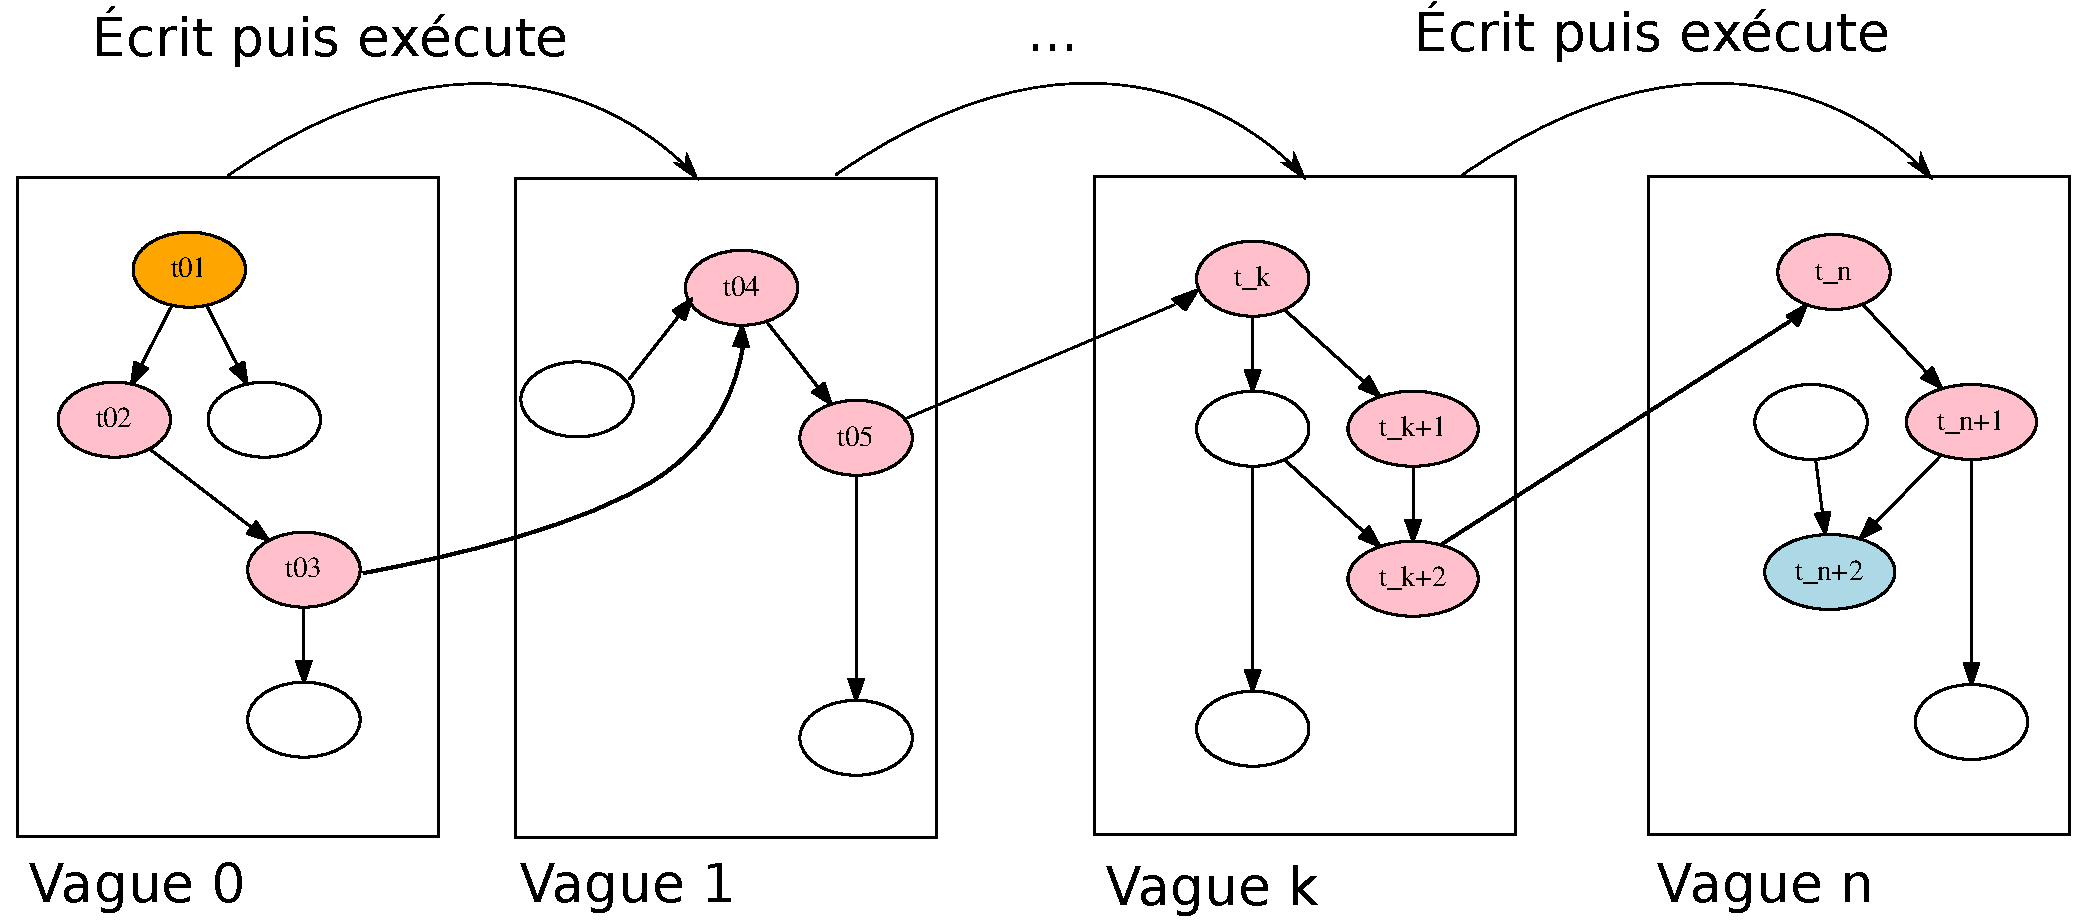
\includegraphics[width=1.0\textwidth]{supports/automodification/phases2_final.pdf}
 \caption{Vision informelle des vagues}
 \label{fig:vagues_visuel}
\end{figure}


\subsubsection{Revue de littérature}
La notion de vague présentée dans ce chapitre a été développée dans les thèse de Calvet \cite{Calvet2013} et Reynaud \cite{Reynaud2010}.
Elle est similaire à la notion de \emph{phase} présentée par Debray et Patel \cite{DP10} et utilisée pour automatiser la suppression de la protection d'un binaire.
En général la suppression des protections se fait à l'aide d'une analyse dynamique et d'une image de la mémoire à un instant donné au cours de l'exécution. C'est cette image mémoire qui sera considéré comme était le programme d'origine. La difficulté réside alors dans le choix de l'instant où prendre l'image mémoire.


\subsubsection{Trace, niveaux d'exécution et vagues}
Le programme exécuté a pour sources principales de données les registres et la mémoire constituée de la pile et du tas qui sont tous les deux adressables par des entiers. Une variable d'un programme est donc soit un registre du processeur soit une adresse mémoire, comme indiqué en définition \ref{def:variable}. Il s'agit du même ensemble $\BV$ que celui défini dans le langage intermédiaire, à la définition \ref{def:sem_conc_var}.
\begin{defi}
On définit l'ensemble $\BV$ des variables comme contenant un ensemble fini de registres $a\in\BA$ et un tableau de taille finie $\mathbb{T}=\textlbrackdbl 0,\ T\textrbrackdbl$.
\label{def:variable}
\end{defi}

En utilisant la sémantique concrète précédemment définie on est capable, à partir d'un ensemble de valeurs initiales pour les registres et la mémoire, d'exécuter un programme sur cette entrée.
Une trace d'exécution d'un programme est simplement l'enchaînement des instructions auxquelles l'exécution du programme a fait appel. Si on note $I_i$ une instruction dynamique, la trace d'exécution est $T=I_1, I_2, ..., I_n$ où $I_n$ est la dernière instruction du programme.

Nous définissons une instruction dynamique (définition \ref{def:ensembles_inst_dyn}) par son adresse, les adresses mémoires sur lesquelles elle est codée et l'instruction machine correspondant. Ces informations sont données par un désassemblage atomique d'une instruction à l'adresse mémoire spécifiée.
Afin de pouvoir séparer la trace d'exécution selon le moment où chaque instruction a été écrite, nous définissons aussi pour chaque instruction l'ensemble des variables sur lesquelles elle provoque une écriture. Cette information est donnée par la sémantique concrète choisie. Avec la sémantique définie à la section précédente les seules instructions qui provoquent des écritures sont celles dont la liste d'instructions atomiques donnée par le désassemblage contiennent des assignation de la forme $x\leftarrow g(x_1, ..., x_m)$ : \dw{D}=\dw{d_1..d_n}=\dw{d_1}$\ \cup\ ...\ \cup\ $\dw{d_n} avec
\\
\dw{d_i}$=
\left\{
  \begin{array}{ll}
	  x &$ si $d_i=x\leftarrow g(x_1, ..., x_m)\ et\ x\in\BV
	\\v &$ si $d_i=x\leftarrow g(x_1, ..., x_m)\ et\ x\notin\BV$: $x=[v]$ est un pointeur vers v$
	\\ \emptyset &$ sinon.$
  \end{array}
\right.
$

\begin{defi}
On note $D$ une instruction dynamique constituée des éléments suivants.
\begin{itemize}
 \item \da{D} l'adresse mémoire de l'instruction dynamique
 \item \dc{D} le segment des adresses mémoire sur lequel \di{D} est codée
 \item \di{D} l'instruction machine à l'adresse \da{D}
%  \item \dr{D_i} l'ensemble des variables sur lesquelles l'exécution de \di{D_i} provoque une lecture
 \item \dw{D} l'ensemble des variables sur lesquelles l'exécution de \di{D} provoque une écriture
\end{itemize}
\label{def:ensembles_inst_dyn}
\end{defi}

Nous avons donc, pour une trace d'exécution donnée, des vagues successives $1, 2, ..., n$.
Au cours de l'exécution du programme on définit, pour chaque adresse en mémoire $m$, un niveau d'écriture $W^M[m]$.
correspondant à la dernière vague $k$ durant laquelle une instruction a modifié la valeur à l'adresse $m$.


Une instruction $D$ a un niveau d'exécution $X$, comme indiqué en définition \ref{def:write_exec_levels}.
Elle a également a un niveau d'écriture $W_D$ qui est le niveau d'écriture le plus élevé parmi les adresses sur lesquelles elle est codée : $W_D=max(W^M[a],\ a\in\ $\dc{D_i}$)$.


\begin{defi}
Nous définissons une trace d'exécution comme la donnée d'une suite $T=t_1, t_2, ..., t_n$ composée de triplets de la forme $t_i=(i, D_i, X_i)$ tels que
\begin{itemize}
 \item $D_i$ est la $i^{eme}$ instruction exécutée.
 \item Avant l'exécution de l'instruction $D_i$, le niveau d'exécution est \texttt{$X_{i-1}$}.
 \item Après l'exécution de l'instruction $D_i$, le niveau d'exécution est \texttt{$X_i$}.
\end{itemize}
\label{def:write_exec_levels}
\end{defi}

\begin{propri}
 Si le niveau d'exécution courant est $X$, le niveau d'exécution de l'instruction à exécuter $D_i$ est :\\
 $X=max(X, W_D+1)$ avec $W_D=max(W^M[a],\ a\in\ $\dc{D_i}$)$.\\
 Après l'exécution de $D_i$, les niveaux d'écriture dans la mémoire sont mis à jour de la manière suivante :\\
 $\forall a\in$ \dw{D_i}, $W^M[a]=X$.
\label{propri:niveau_exec}
\end{propri}

En pratique une instruction $D$ écrite par une instruction ayant pour niveau d'exécution $k$ puis directement exécutée aura pour niveau d'écriture $W_D=k$ et pour niveau d'exécution $X=k+1$. Ce comportement est formalisé par la propriété \ref{propri:niveau_exec}.

On définit alors formellement la vague $k$ selon la définition \ref{def:vagues} et l'algorithme \ref{algo:analyse_dyn_vagues} permet d'exécuter un programme dynamiquement avec la sémantique concrète choisie tout en déterminant les niveaux d'exécution de d'écriture au fur et à mesure de l'exécution. La sortie de l'algorithme \ref{algo:analyse_dyn_vagues} est la trace d'exécution et la liste des vagues reconstruites.
\\

Reprenons l'exemple du programme auto-modifiant de la figure \ref{fig:unevague_trace}.
La figure \ref{fig:unevague_trace} donne une trace d'exécution de ce programme en détaillant les informations sur chaque instruction dynamique ainsi que les niveaux d'écriture et d'exécution de chaque instruction.
Au départ toute la mémoire est dans son état d'origine et a pour niveau d'exécution 0. Lorsque l'instruction $D_0$ est exécutée, il n'y a pas eu d'auto-modification donc le niveau d'écriture est 0 et le niveau d'exécution est 1.
Les instructions $D_3$ et $D_4$ provoquent une auto-modification : les octets aux adresses \adr{0x8048091} et \adr{0x8048092} sont modifiés et leurs niveaux d'écriture deviennent donc le niveau d'exécution courant, soit 1.
Lorsque l'exécution atteint $D_5$, qui a été modifié, le niveau d'écriture est 1 donc le niveau d'exécution devient 2.
L'instruction suivante $D_6$ fixe la valeur de \edi\ à 2 puis les instructions suivantes provoquent l'affichage de \edi.

Cette trace d'exécution est donc composée de deux vagues : la vague initiale, $v_0$ composée de l'état de la mémoire avant l'exécution de la première instruction et la vague $v_1$ contenant l'état de la mémoire juste après l'exécution de $D_4$ et avant l'exécution de la première instruction modifiée $D_5$.




\begin{defi}
 Étant donné une trace d'exécution $T=t_1, ..., t_n$ avec $t_i=(i, D_i, X_i)$ et $k\in\{X_j, 1\leq i\leq n\}$, on appelle vague $k$ l'état de la mémoire juste après l'exécution de la dernière instruction ayant pour niveau d'exécution $k$.
 C'est à dire l'état de la mémoire juste après l'instruction $D_j$ avec $X_{j+1}>k$.
 \label{def:vagues}
\end{defi}

% \begin{algorithm}[H] %or another one check
% \caption{Mise à jour des niveaux d'exécution et d'écriture lors de l'exécution d'une instruction}
% \SetAlgoLined
% \KwIn{La mémoire, l'opérateur de niveau d'écriture, une instruction dynamique et le niveau d'exécution courant}
% \KwResult{L'opérateur de niveau d'écriture et le niveau d'exécution courant mis à jour}
% \SetKwProg{Fn}{}{}{}
% \SetKwFunction{FRecurs}{calculNiveau}
% \Fn(
% ){\FRecurs{M, $W^M$, D, X}}{
% $W_D \leftarrow\ max(W^M[a],\ a\in\ $\dc{D}$)$\\
% $X \leftarrow\ max(X,\ W_D+1)$ \\
% \For {$m\in\ $\dw{D}}{
%   $W^M[m]\leftarrow\ X$
% }
% \Return ($W^M$, X)
% }
% \label{algo:update_vagues}
% \end{algorithm}

\begin{algorithm}[H] %or another one check
\caption{Mise à jour du niveau d'exécution d'une instruction}
\SetAlgoLined
\KwIn{La mémoire, l'opérateur de niveau d'écriture, une instruction dynamique et le niveau d'exécution courant}
\KwResult{Le niveau d'exécution courant mis à jour}
\SetKwProg{Fn}{}{}{}
\SetKwFunction{FRecurs}{MAJExecution}
\Fn(
){\FRecurs{M, $W^M$, D, X}}{
$W_D \leftarrow\ max(W^M[a],\ a\in\ $\dc{D}$)$\\
$X \leftarrow\ max(X,\ W_D+1)$ \\
\Return X
}
\label{algo:update_exec_level}
\end{algorithm}

\begin{algorithm}[H] %or another one check
\caption{Mise à jour des niveaux d'écriture lors de l'exécution d'une instruction}
\SetAlgoLined
\KwIn{La mémoire, l'opérateur de niveau d'écriture, une instruction dynamique et le niveau d'exécution courant}
\KwResult{L'opérateur de niveau d'écriture mis à jour}
\SetKwProg{Fn}{}{}{}
\SetKwFunction{FRecurs}{MAJEcriture}
\Fn(
){\FRecurs{M, $W^M$, D, X}}{
\For {$m\in\ $\dw{D}}{
  $W^M[m]\leftarrow\ X$
}
\Return $W^M$
}
\label{algo:update_write_level}
\end{algorithm}

\begin{figure}
\begin{center}
\begin{tabular}[b]{|l|l|l|l|l|l|l|}
\hline
i & \da{D_i} & \dc{D_i} & \di{D_i} & \dw{D_i} & $W_i$ & $X_i$ \\
\hline
& 8048060  &  (...)         	        & Pile -> RWX &  & 0 & 1 \\ 
1 & 804807c  &  [804807c, 8048080]         &  mov    edi, 0x0 & edi & 0 & 1 \\
2 & 8048081  &  [8048081, 8048086]         &  mov    eax, 0x8048091 & eax & 0 & 1 \\
3 & 8048086  &  [8048086, 804808a]         &  mov    [eax], 0xeb & 0x8048091 & 0 & 1 \\
4 & 804808b  &  [804808b, 8048090]         &  mov    [eax+1], 0x7 & 0x8048092 & 0 & 1 \\
5 & 8048091  &  [8048091, 8048092]         &  jmp    80480a1 <edi3> &  & 1 & 2  \\
6 & 804809a  &  [804809a, 804809d]         &  mov    edi,0x2 & edi & 0 & 2\\
7 & 804809f  &  [804809f, 80480a0]         &  jmp    80480a8 <fin> &  & 0 & 2\\
 & 80480a8  &  (...)		        &  Affiche edi &  & 0 & 2\\
 & 80480c3  &  (...)		        &  Quitte &  & 0 & 2\\
\hline
\end{tabular}
\end{center}
\caption{Trace d'exécution du programme auto-modifiant de la figure \ref{fig:unevague_v0}}
\label{fig:unevague_trace}
\end{figure}

\begin{algorithm}[H] %or another one check
\caption{Analyse dynamique avec calcul des vagues}
\SetAlgoLined
\KwIn{Les registres R et une mémoire M dans laquelle un programme a été chargé à son point d'entrée \texttt{ep}}
\KwResult{La trace des instructions dynamiques chacune associée à leur niveau d'exécution et les différentes vagues de la trace}
\SetKwProg{Fn}{}{}{}
\SetKwFunction{FRecurs}{analyseDynamique}
\Fn(
% \tcc*[h]{C : matrice des associations possibles, i : numéro du prochain sommet de P à associer, F : liste des couples d'associations déjà faites}
){\FRecurs{R, M, ep}}{
\For{$m\in M$}{
  $W^M[m]\leftarrow 0$\\
}
$X\leftarrow 1$\\
$X_{-1}\leftarrow 0$\\
$i\leftarrow 0$\\
$T\leftarrow \emptyset$\\
$vagues\leftarrow \emptyset$\\
$eip\leftarrow ep$\\
\While {la fin du programme n'est pas atteinte} {
$i\leftarrow i+1$\\
~\\
$D\leftarrow decode(eip, M)$\\
$X\leftarrow MAJExecution(M, W^M, D, X)$\\
\If {$X \ne X_{-1}$}{
  $vagues\leftarrow vagues\cup \{(X_{-1}, M)\}$
}
$X_{-1} \leftarrow X$\\
~\\
$(eip, R, M)\leftarrow sem\_eval(eip, R, M)$\\
$W^M\leftarrow MAJEcriture(M, W^M, D, X)$\\
$T\leftarrow T\cup\{(i, D_i, X)\}$\\
}
\Return T, vagues
}
\label{algo:analyse_dyn_vagues}
\end{algorithm}

\begin{rem}
 Étant donné la définition croissante des vagues, la même instruction $D$ peut-être exécutée non seulement plusieurs fois dans la même vague mais également être présente à des vagues différentes.
\end{rem}

\subsection{Implémentations}
\todo[inline]{émulation VS instrumentation VS déboguage}
\todo[inline]{BAP: \\
Jakstab: \\
TraceSurfer: (outil de daniel)\\
Renovo : \\
LLVM : (pk ne pas l'utiliser??) \\
Implem en C: \\
Pin : \\
Xed : \\
}
\subsection{Revue de littérature}
\subsection{Émulation avec BAP}
\subsection{Instrumentation avec Pin}
\section{Analyse statique et chevauchement de code}
\section{Codisasm}